
%===============================================================================
\chapter{Framework1}\label{Kap:Frame1}
% 10.06.2020
% Stefan Briem
% ===============================================================================
%Benötigte plots aus matlab:
% 1-5 Anchor-Boxen
% Traninglos (eventuel Die passende Training-Udates tabelle dazu)
% ===============================================================================
In diesem Kapitel wird das erste sogenannte ''Framework'' des ersten Teils des Projektes beschrieben. Wenn man hier vom ersten Teil spricht, ist die logische Arbeitsaufteilung des Netzwerkes in die \textbf{Erstellung} und den \textbf{Einsatz} des KNN gemeint. Somit geht es in diesem Kapitel um die \textbf{Erstellung} beziehungsweise das Designen und Trainieren eines KNN.\\
Für eben dieses Framework wurde ein Matlab-Livescript namens ''yolov2\_Framework1.mlx'' erstellt. Ziel dieses Livescripts war es, den benötigten Code bereitzustellen und zu implementieren. Der Anspruch dabei war, dass die Vorgänge reproduzierbar sein sollten. Das heißt, dass im Nachhinein nachvollzogen werden kann, welche Daten und Einstellungen verwendet wurden. Außerdem muss es auch möglich sein durch einen einfachen Ausführ-Befehl (drücken auf 'Run') das Script oder die einzelnen Skript-Teile auszuführen. Dies alles mag sich wie selbstverständlich und simpel anhören, da beim Trainieren jedoch auf Datensätze, wie Bilder und Label- Datensätze zugriffen wird und diese Daten auch noch angepasst werden müssen, ist diese Aufgabe durchaus sehr arbeitsintensiv, jedoch gleichzeitig für das weitere Vorgehen unverzichtbar. \\
Zudem wurde das Livescript so geschrieben, dass es interaktiv und gut zu bedienen ist. Oberhalb der jeweiligen Programmabschnitte wird zusätzlich kurz beschrieben was jeweils nachfolgend implementiert ist. \\
\newline


\section{Beschaffen der Trainingsdaten}
zum Ausführen des Lifescripts werden Trainingsdaten benötigt. Beschaffung wird hier beschrieben
\subsection{Bilder und Videos}

\subsection{Label}\label{sec:Frame1Label}
==>>supervised Learning deshalb müssen Label erstellt werden.\\
aufbau eines LAbels [1 2 3 4]

\subsection{Image-Labeler} \label{sec:Frame1ImageLabeler}
\subsection{Video-Labeler}


\section{Livescript-Beschreibung}

\textcolor{red}{KMT hab erst hier wieder weitergemacht\newline}Mit diesem Livescript kann, mithilfe bereits gelabelter Bilder ein Neuronales Netzwerk erstellt, trainiert und evaluiert werden. Dazu sind abhängig von den jeweiligen Anforderungen verschiedene Schritte notwendig. Das Livescript soll dabei interaktiv nutzbar sein und möglichst alle Aufgabenstellungen, die bei vorliegendem Projekt in diesem Teil auftauchen können, abdecken. Das Livescript kann so genutzt werden, dass bestimmte Aktionen, je nach Bedarf entsprechend ausgeführt werden können oder eben auch nicht. Es geht also nicht darum immer das ganze Skript auszuführen.  An verschiedenen Stellen können Aktionen auf verschiedene Art und Weise oder mit wählbaren Parameters oder anderen Datensätze durchgeführt werden.\\
Im diesem Abschnitt der Dokumentation wird dieses Livescript beschrieben. Diese Beschreibung orientiert sich an der Struktur des Skriptes.  So ist die Section x. y) im Livescript hier im Unterpunkt x. y) beschrieben, wobei die jeweiligen Hintergründe und erforderlichen Variablen erklärt werden. Dies ermöglicht eine sehr einfache und intuitive Hilfe bei der Anwendung des vorliegenden Codes. \\
Das Framework (und damit auch das Livescript) besteht aus folgenden 3 Hauptteilen:
\begin{enumerate}
	\setlength{\itemsep}{-1ex}
	\item{\begin{flushleft} \textbf{Daten einlesen und aufbereiten} \end{flushleft}}
	\item{\begin{flushleft} \textbf{Trainieren} \end{flushleft}}
	\item{\begin{flushleft} \textbf{Trainiertes Netzwerk testen und evaluieren} \end{flushleft}}
\end{enumerate}

\subsection{Daten einlesen und Aufbereiten}
Der erste Teil des Livescripts beschäftigt sich mit dem Laden und Aufbereiten der für das Training benötigten, Datensätze.
\subsubsection{a) Laden der Labels und Pfade}
Wie bereits oben angedeutet, müssen verschiedene Datensätze geladen werden. Um dies zu gewährleisten, wurde eine Ordnerstruktur eingerichtet. Sie besteht aus folgenden Ordern
\begin{enumerate}
	\setlength{\itemsep}{-1ex}
	\item{\textbf{''Bilder'':}} In diesem Ordner sind die Bilder-Sätze, auf die das Netzwerk für das Training zugreift, in Unterordnern abgespeichert. Diese Bilder sind auf die Auflösung, die das Netzwerk benötigt skaliert.
	\item{\textbf{''Labels'':}} Hier sind die Label in '.mat' Dateien abgespeichert
	\item{\textbf{''LabelSessions'':} } Für die Erstellung der Label wird die App ''ImageLabeler'' (siehe Abschnitt \ref{sec:Frame1ImageLabeler}) verwendet. Von dort aus können die Label in den Ordner ''Labels'' exportiert werden. Um diese später jedoch weiter verändern zu können, kann aber auch einfach die Label-Session gespeichert und später wieder mit dem ''ImageLabeler'' geöffnet werden.
	\item{\textbf{''MatlabCode'':}} Hierauf muss der Matlab-Pfad gesetzt sein. Sowohl das Livescript, als auch die von ihm aufgerufenen Matlab-Functions befinden sich in diesem Ordner.
	\item{\textbf{''NeuronaleNetzwerke'':}} Hier befinden sich Matlab-KNN die importiert werden. Dieser Ordner ist zur Zeit nicht verwendet.
	\item{\textbf{''OriginalBilder'':}} In diesem Ordner befinden sich die Original Bilder-Sätze in ihrer ursprünglichen Auflösung (Größe).
	\item{\textbf{''TrainedDataWorkspaces'':}} Hier werden die Detektoren abgespeichert (siehe Abschnitt \ref{sec:Frame1TrainierenSaveDetector}). 
\end{enumerate}
Diese gesamte Ordnerstruktur kann nun kopiert und auf anderen PC ausgeführt werden.
\textbf{Achtung:} Da Matlab beim Zugriff auf Dateien mit Pfaden in String-Format arbeitet, müssen die OrdnerNamen genau so geschrieben werden.\\

Um späteres Zugreifen auf die Ordner der Struktur zu gewährleisten wird die Funktion ''fileparts'' ausgeführt. 	
\begin{matlabcode}
		[f1,f2,f3]=fileparts(pwd) % Determinieren des aktuellen (gesamten) Pfades
	\end{matlabcode} 
Der Inhalt der zurückgegebenen Variablen:
\begin{matlabcode}
	 f1 = String des Pfades des Übergeordneten Ordners
	 f2 = String des untersten angwählten Ordners (hier'MatlabCode')
	 f3 = 0x0 empty char array (Wird nicht weiter verwendet)
\end{matlabcode}

\subsubsection{b) Konfigurieren der Datensätze}
In diesem Teil werden die Datensätze konfiguriert. Dazu stehen dem Anwender sechs Auswahlmöglichkeiten in Form von Fragen zur Verfügung. Diese kann Er entweder über eine Checkbox mit ''true'' oder ''false'' beantworten, oder über eine Dropdown-Liste eine Antwort auswählen.  	
	\begin{enumerate}
		\item{ Werden skalierte Bilder oder die Originalbilder verwendet? }  						(Checkbox)
		\item{ Sollen bereits skalierte Bilde verwendet werden oder müssen Bilder neu-skaliert werden? }  (Checkbox)
		\item{ Werden eigene Bilder oder Matlab-Bilder verwendet? }  								 (Dropdown)
		\item{ Welcher Bilder-Datensatz ist gewünscht?  }   									(Dropdown)
		\item{ Welche Label sollen verwendet werden auswählen? } 									 (Dropdown)
		\item{ Welches Objekt soll detektiert werden?  }   											(Dropdown)
	\end{enumerate}
Je nach Auswahl werden die entsprechenden Pfade geadded und die Label geladen.
	
\subsubsection{c) Erstellen von 'TrainingData'}	 \label{sec:Frame1TrainingData}
Hier werden die Daten der Label mit den passenden Dateipfaden versehen. Dabei wird sowohl eine Tabelle mit den Pfaden der Original-Bilder, als auch eine Tabelle mit den Pfaden der skalierten Bildern erstellt.\\
\textbf{Achtung:}  Der Funktion ''objectDetectorTrainingData()'' wird der Inhalt der entsprechenden Label-Datei in einem Matlab-spezifischen Datentyp namens 'gtruth' übergeben. Befinden sich in der Label-Datei leere Bilder, also Bilder in denen keine Objekte gelabeled wurden, so werden diese verworfen. Die Variable 'NumberOfPictures' besagt also nicht wie viele Bilder im Datensatz sind, sondern nur wie viele Bilder aus diesem Datensatz in der Label-Session mit mindestens einem Label versehen geworden sind.\\
	
\begin{matlabcode}
	trainingData = objectDetectorTrainingData(gTruth);
	[NumberOfPictures,i]=size(trainingData)   %  NumberOfPictures = 355  
\end{matlabcode}

\subsubsection{d) Skalieren der Bilder/Videos mit den zugehörigen Bounding Boxes:}
Jedes trainierte Netzwerk ist auf eine bestimmte Bildgröße ausgelegt. Für die Effektivität des Netzwerkes ist es von Vorteil, manchmal sogar essentiell, die Bildgröße (Bildauflösung) an das KNN anzupassen. Außerdem sollen die Trainierten Netzwerke perspektivisch auch auf dem Raspberry-Pi und einer passenden Webcam ausführt werden. Daher macht es Sinn, dieselbe Auflösung zu verwenden da sonst Training und Anwendung nicht zusammen passen. Die Webcam hat jedoch nicht die Auflösung einer normalen Consumer-Kamera.
Für das spätere Abgleichen und Testen des Netzes mit Kameras an bekannten Bildern, die auf dem Bildschirm angezeigt werden, ist es jedoch vorteilhaft hochauflösende und damit realitätsnähere Bilder zu benutzen. Daher sind Hochauflösenden Bilder insbesondere für das Testen und Abgleichen und die skalierten Bilder für das Trainieren geeignet.\\
Deshalb gibt es im Framework die Möglichkeit Bilder auf die gewünschte Größen zu skalieren. Da die Label auch in Pixel Einheiten beschrieben werden (siehe Abschnitt \ref{sec:Frame1Label} ), müssen auch die Label der Bildern skaliert werden. \\

Zuerst wird über die Variable ''useScaledPictures'' abgefragt, ob für das Training skalierte Bilder benutzt werden sollen oder nicht. Falls skaliert werden muss, wird über die Variable ''maxSize'' die Pixelzahl des skalierten Bildes an der langen Kante festgelegt. Das eigentliche Skalieren wird in der selbstgeschriebene Funktion ''scale\_images\_and\_labels'' durchgeführt. Hierbei werden die skalierten Bilder in den bereits beschriebenen Ordner abgelegt.  Die genau Funktionsweise ist in den Kommentaren der gleichnamigen Matlab-Function festgehalten.  \\\textcolor{red}{KMT evtl noch beschreiben, mal sehen wies am ende aussieht...}
Der Funktion muss Folgendes übergeben werden :
\begin{enumerate}
	\item \textbf{'trainingDatenOriginal':} Enthält die Pfade der Originalbilder. So können die Originalbilder eingelesen werden.  
	\item \textbf{'trainingDatenCopy':}  Wird als der in Abschnitt \ref{sec:Frame1TrainingData} beschriebene Trainingsdatensatz der Skalier-Funktion übergeben. Die Label werden in der Funktion skaliert und anschließend dem Datensatz zurückzugeben
	\item  \textbf{'maxSize':} Die gewünschte maximale Kantenlänge des skalierten Bildes in Pixeln.
	\item  \textbf{'labeledObject':} Auf dieses Objekt soll das Netzwerk trainiert werden. (Nur die Label dieses Objektes werden skaliert)   
\end{enumerate}


\begin{figure}[h]
\begin{tiny}
	\begin{matlabcode}
		if useScaledPictures         % werden skalierte Bilder benutzt  
			
			trainingDataCopy    = trainingData;
			trainingDataBackup  = trainingData;    
			maxSize             = 200   
			trainingDataCopy     = scale_images_and_labels(trainingDataOriginal,trainingDataCopy,maxSize,scalePictures,labeledObject);   
			trainingData        = trainingDataCopy;
			clear trainingDataCopy;
		
		else
		
			clear trainingDataOriginal;  
	
		end
	\end{matlabcode}
\end{tiny}	
\caption{Livescript Matlab-Code zum Skalieren der Trainingsdaten}
\end{figure}
	
\subsubsection{e) Eliminieren der ungenutzten Bilder und Label}
In Abschnitt \ref{sec:Frame1TrainingData} werden die Bilder ohne Label bereits aus dem Trainingsdatensatz entfernt. Dort wurden jedoch nur die Bilder ohne \textbf{jegliche} Label eliminiert. Da das Netzwerk aber nur auf \textbf{ein} Objekt trainiert wird, werden hier sowohl alle Label anderer Klassen, als auch die Bilder, die keine Label der gewünschten Klasse besitzen, entfernt.
	
\subsubsection{f) Weiteres aufbereiten der Daten:} \label{sec:Frame1CreateDatastore}
Hier werden die Trainingsdaten in einen anderen Matlab-spezifischen Datentyp, dem sogenannten ''Datastore'' der später der Trainingsfunktion übergeben wird, konvertiert.

\subsubsection{g) Mischen der Bilder: (optional)}
Falls gewünscht, können hier die Trainingsdaten gemischt werden, sodass die Tabelle der Trainingsdaten nicht mehr nach den Namen der Bilder geordnet ist. Es ist jedoch zu beachten, dass beim Trainieren die Bilder auch ständig gemischt werden. Tatsächlich werden randomisierte Gruppen von Bildern trainiert (sogenannte Minibatches siehe Abschnitt \ref{sec:Frame1TrainingOptions}).\\
Dieses Mischen hat also eigentlich nur Auswirkungen auf das spätere Auswerten der Bilder. De facto benötigten wir diese Funktion nicht, es kann aber gut sein das zukünftige Anforderungen auftauchen, bei denen ein Misch-Vorgang hilfreich sein kann. Deshalb ist dieser Abschnitt hier implementiert.

\subsubsection{h) Visualisierung}
Nachdem der Trainingsdatensatz nun aufbereitet ist, wird nun dem Bediener ein Überblick über eben diese Trainingsdaten gegeben. \\
Der Befehl ''summary(trainingData)'' zeigt die Anzahl der Bilder und den Namen des zu detektierenden Objektes an.\\
Durch das Separieren der Bounding-Boxes (Größe und Position der Label) wird das Objekt ''allboxes'' erzeugt. Die Dimension diese Objektes zeigt die Anzahl der Bounding-Boxes. \\
Das Seitenverhältnis ('aspectRatio') und die Fläche('area') der Bounding-Boxes werden in einem Scatter-Plot dargestellt(siehe Abbildung \ref{fig:Frame1BoundingBoxes}). Mit Hilfe dieses Plots, kann sich der Anwender einen Überblick über die Größe und Form der Label und deren Streuung \textcolor{red}{KMT}beschaffen.

\begin{figure}
	\begin{center}
		\includegraphics[width=0.7 \textwidth]{./figures/figure_0.png}
		\caption{Scatter-Plot des Label-Satzes 'pictures0014' aus 'collection1'}
		 \label{fig:Frame1BoundingBoxes}
	\end{center}
\end{figure}

\subsubsection{i) Label Überprüfung}
Bei der Erstellung der Label können leicht fehlerhafte Label produziert werden. Überschreitet ein Label zum Beispiel die Bildränder, so funktioniert das Trainieren nicht mehr. Es kann auch vorkommen, dass beim Zeichnen der Label durch einen Klick zu viel ein 'Fake-Label', das sehr klein ist und deshalb übersehen wird, entsteht. Die manuelle Fehlersuche stellte im Verlauf des Projektes ein echtes Problem dar. \\
Hinzu kommt, dass durch das Skalieren beispielsweise kleine Objekte sehr unscharf werden und damit nicht mehr brauchbar sind. Zu guter Letzt kann es auch von Vorteil sein, ein Netzwerk nur auf eine bestimmte Objekt-Größe zu trainieren.\\
All dies stellt nicht ein einmalig auftretende Problem dar, sondern wird immer wieder auftauchen. Zum Beispiel durch neue Datensätze, angepasste Anforderungen oder auch dem Deployen des Codes auf einen Raspberry-Pi als Target.\\
Die selbstgeschriebene Funktion 'checkLabels' überprüft die Label auf die gegebenen Standards. Dabei kann eine maximale und ein minimale Größe der Fläche in Pixeln festgesetzt werden. Außerdem überprüft die Funktion, ob ein Label die Bildränder überschreitet. Kommt es zu einem Regelverstoß, so wird das entsprechende Bild geplottet und der 'Regelverstoß' angezeigt. 
Abbildung \ref{fig:Frame1PictureToSmall} zeigt einen solchen Plot. In diesem Beispiel ist auch zu erkennen, dass das zu detektierende Objekt bei dieser Auflösung eigentlich nicht mehr zu erkennen und das Label somit nicht brauchbar ist.\\
Am ende des Label-Checks plottet die Funktion ein Bild mit den zugehörigen Label(Abbildung \ref{fig:Frame1Stichprobe}). Somit kann überprüft werden, ob Label- und Bild-Datensätze zusammenpassen (richtiges Label im richtigen Bild), und ob die Skalierung der Bilder und Label funktioniert hat.

\begin{figure} 
		\begin{center}
	\includegraphics[width=0.7 \textwidth ]{./figures/figure_1.png}
	\caption{Beispiel eines als zu klein befundenen Labels. Matlab wird den Text 'A Bounding-Box in Picture18 is to small' dazu ausgeben.}
	\label{fig:Frame1PictureToSmall}
		\end{center}
\end{figure}

\begin{figure}
	\begin{center}
		\includegraphics[width=0.7 \textwidth]{./figures/figure_49.png}
		\caption{Das Bild zeigt, die am Ende des Label-Checks geplottete, Stichprobe.}
		\label{fig:Frame1Stichprobe}
	\end{center}
\end{figure}
	
\subsection{Trainieren}
Der  zweite Teil des Frameworks beschäftigt sich mit dem Training des Netzwerkes. Dazu gehört sowohl der Trainingsvorgang an sich, als auch das Setzen der Trainingsparameter, sowie das Abspeichern des trainierten Netzwerkes und das Visualisieren des Trainingsvorganges.

\subsubsection{a) Determinieren/auswählen der Bounding-Boxes}
Hierbei geht es darum, die sogenannten Anchor-Boxes zu bestimmen. Diese Anchor-Boxes sind ein entscheidender Parameter beim Trainieren eines Netzwerkes und entsprechen in ihrem Format Label (bzw. Bounding-Boxes) ohne feste Ortsangabe(verschiebbare Fenster). Sie sind also einfach durch Länge und Breite beschrieben. Man versucht nun aus den Eigenschaften der Label, des Trainings-Datensatzes die Anchor-Boxes und deren Eigenschaften zu determinieren. Hierbei geht es um die Größe und das Seitenverhältnis der Bounding-Boxes (bzw. der daraus resultierenden Anchor-Boxes). 
Je breiter die Streuung der Bounding-Boxes hinsichtlich dieser Eigenschaften ist, desto schwerer ist es, diese Eigenschaften mit wenigen Anchor-Boxes abzubilden. Um dies zu visualisieren,  wird  hier im 1. Schritt deren  ''Abdeckrate'' in Abhängigkeit von der Anzahl an Anchor-Boxes aufgetragen. Diese beschreibt, in welchem Maße die Gesamtheit aller Boxes mit möglichst wenigen möglichst gut zusammenfassen lässt. Diese ''Abdeckrate'' nennt Matlab ''meanIoU''. Diese Variable ist auf 1 (entspricht 100\% Abdeckrate) normiert und sollte auf jeden Fall größer als 0.5 sein. Eine größerer Anzahl an "Ankern"(Anchor-Boxes) führt oft zu einer höheren Abdeckrate und verbessert somit die Performance des Netzes. Eine zu große Anzahl an Anchor-Boxes kann aber auch den Rechenaufwand unverhältnismäßig erhöhen und außerdem zur Überanpassung (Overfitting) führen. Bei einer Überanpassung wird das Netzwerk zu stark speziell auf den Datensatz trainiert und kann deshalb Objekte in leicht abweichenden Testdaten nicht mehr erkennen. Zudem ist für eine größere Anzahl an Anchor-Boxes ein größeres und tieferes Netzwerk vonnöten. Deshalb muss der Bediener für das Training seines Netzwerkes selbst abwägen und entscheiden wie viele Anchor-Boxes er benutzen möchte. Dieses Vorgehen ist nicht nur deterministisch sondern in großen Teilen empirisch.\\
\begin{figure}
	\begin{center}
		\includegraphics[width=0.7 \textwidth ]{./figures/figure_51.png}
	\end{center}	
	\label{fig:frame1MeanIoU}
	\caption{Abdeckrate ''meanIoU'' in Abhängigkeit Anchorbox-Anzahl für Datensatz'pictures0014' und den Label vom Typ ''car''}
\end{figure}
Für das in Abbildung \ref{fig:frame1MeanIoU} dargestellte Beispiel wäre beispielsweise eine Anzahl von Anchor-Boxes von 4 bis 8 passend. Bei der Anzahl der Anchor-Boxes ist man manchmal auch durch das bereits vortrainierte KNN eingeschränkt. Dies haben oft eine maximale Anzahl an möglichen Anchor-Boxes. Wie oben bereits beschrieben, geht es nicht darum die höchstmögliche Abdeckrate zu erreichen, sondern um einen Trade-Off zwischen dem Traininings-Aufwand und der Gefahr der Überanpassung des Netzwerkes mit einer möglichst hohen Abdeckrate.\\
\newline
Nachdem die Anzahl der Anchor-Boxes bestimmt wurde, wendet man darauf die Funktion ''estimateAnchorBoxes'' nochmals an. Diesmal geht es nicht primär um die Anzahl sondern stattdessen um die Größe und das Seitenverhältnis der Anchor-Boxes.\\ 
Um dies nochmals graphisch zu verdeutlichen sind in Abbildung \ref{fig:Frame1DifferentAnchorNumbers} die verschiedenen Anchor-Boxes über Fläche und Seitenverhältnis, in Abhängigkeit der gewählten Anzahl der Anchor-Boxes, dargestellt.\\
Abbildung \ref{fig:Frame1FinalAnchorOverLabel} zeigt, das bereits in Abbildung \ref{fig:Frame1BoundingBoxes} visualisierte Beispiel mit den darüber gelegten Anchor-Boxes in grün. Diese Visualisierung kann dabei helfen zu verstehen welche Label wohl durch die Bounding-Boxes nicht abgedeckt werden. Dies hilft wiederum  die Einstellungen anzupassen oder das Verhalten beziehungsweise die Zuverlässigkeit des trainierten Netzwerkes besser zu verstehen.\\
Die Abbildung \ref{fig:Frame1DifferentAnchorNumbers} zeigt die Anordnung der Anchor-Boxes in Abhängigkeit der gewählten AnchorBox-Anzahl.
	
\begin{figure}[h]
	\begin{center}
	\includegraphics[width=0.7 \textwidth]{./figures/figure_52.png}
	\end{center}
	\label{fig:Frame1FinalAnchorOverLabel}
	\caption{Vier Anchor-Boxen im Label-Satz 'pictures0014' aus 'collection1'}
\end{figure}	

\begin{figure}[h]
	\begin{center}
		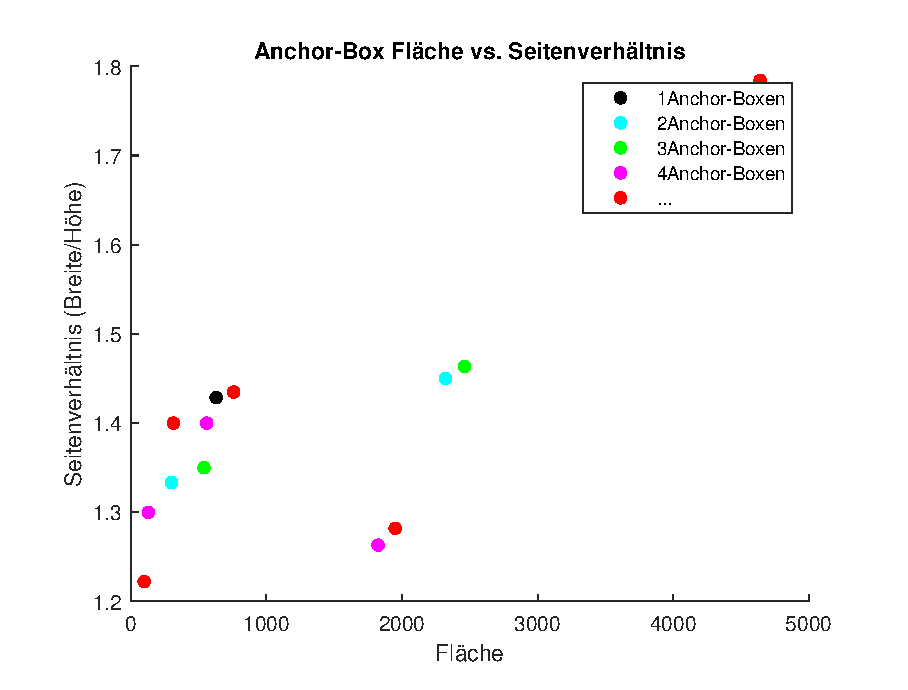
\includegraphics[width=0.7 \textwidth]{./figures/figure_2.eps}
	\end{center}
	\label{fig:Frame1DifferentAnchorNumbers}
	\caption{Verschiedene Anchor-Box-Anzahlen für den Label-Satz 'pictures0024' aus 'collection1'}
\end{figure}
\newpage
\subsubsection{b)Laden des vortrainierten Netzwerkes mit anschließendem Manipulieren/Verändern} \label{sec:Frame1Lgraph}
Bei der Bestimmung des KNN sind hier drei Optionen vorgesehen. 
\begin{enumerate}
	\item Wählt man im Dropdown der Variable ''network'' die Option \textbf{''small''} aus, wird ein relativ kleines Netzwerk mit 25 Layern geladen. An dieses Netzwerk können, durch die interne Struktur des Netzwerkes bedingt, nur maximal 4 Anker Boxen übergeben werden. Die passende  'ImageSize' ist 128x128x3
	\item Wählt man 'Resnet50', so wird das sehr große Netzwerk \textbf{''resnet50''} über eine Matlab-Funktion geladen. Diese Funktion ist also nicht lokal gespeichert, sondern eine Vor-implementierte Matlab-Funktion. Dieser Funktion können die Parameter zur Bildgröße, zur Anzahl der Klassen (hier immer 1), die Anker-Boxen, die Aktivierungsfunktion und der Name eines Netzes übergeben. Der Netzname ist hier ''resnet50''.
	\item Die Option \textbf{''resnet50SelfApplied''} lädt im Prinzip das Netzwerk aus Option 2 im Stil von Option 1. Die Aufgerufene Funktion ist also auch lokal abgespeichert und kann verändert werden.   
\end{enumerate}
Bei allen drei Optionen wird die Variable 'lgraph' zurückgegeben. Sie ist von einem Matlab eigenen Datentyp und wird in Abschnitt  \ref{sec:Frame1Training} der Funktion, die den Trainingsvorgang ausführt, übergeben.

	
\subsubsection{c)Einstellen der ''trainingOptions''} \label{sec:Frame1TrainingOptions}
Bevor das Training des KNN beginnen kann, müssen noch die Optionen des Trainings festgelegt werden. Bis jetzt wurde nur die Netzstruktur festgelegt. Jetzt muss auch noch bestimmt werden,wie die Internen Parameter angepasst werden sollen. Natürlich handelt es sich prinzipiell um ein Gradient-Descent Verfahren. Das heißt, die Abweichung zwischen dem durch die Trainingsdaten vorgegebenen Optimum und dem Ergebnis des Netzwerks stellt den Fehler da. Durch die Bestimmung des aktuellen Gradienten (Steigungstangente in mehreren Dimensionen) wird die Richtung bestimmt. Das Netzwerk verändert seine Parameter dieser Richtung entsprechend und kommt so dem Optimum etwas näher. \\
Es muss jedoch gewählt werden, wie die Daten eingesetzt werden, wie groß die Schrittweite ist, wie intensiv trainiert werden soll usw..
Außerdem nutzen die eingesetzten Verfahren natürlich einige Kniffe um numerische Effekte und ähnliches zu eliminieren.

\begin{itemize}
	\item \textbf{'sgdm'}:Stochastic-Gradient-Descent Optimierung. Das 'm' steht für Matlab. Hierbei handelt des sich um ein spezielles Gradient-Descent Verfahren.
	\item \textbf{'InitialLearnRate'}: Ist ein Maß für die Größe der Gradienten-Schrittweite einer Iteration.
	\item \textbf{'Verbose'}: Es handelt sich um eine binäre Variable. Ist Sie auf 'true' gesetzt, so werden die Zwischenergebnisse des Trainingsvorganges, wie in Tabelle \ref{tab:Frame1Tainingsvorgang} dargestellt, im Live-Script ausgegeben.(siehe Abschnitt \ref{sec:Frame1Training})
	\item \textbf{'MinibatchSize'}: Numerisch ist es nicht sinnvoll die Forward- und Backprogagation jeweils für den ganzen Datensatz zu machen. Stattdessen wird der Datensatz in sogenannte 'Minibatches''(Bild-Gruppen) aufgeteilt. Mit jeder dieser Minibatches wird dann jeweils eine Forward- und Backprobagation durchgeführt. Sowohl am Anfang als auch jedes mal nach dem Durchlauf aller Minibatch-Blöcke durch das Netzwerk. Werden diese Minibatches neu gewürfelt. In den Optionen kann nun also die Größe der Minibatch festgelegt werden.\\
	\textbf{Tipp}: Erfahrungen haben gezeigt, dass es beim ersten Trainieren eines KNN sinnvoll ist die 'MinibatchSize' realtiv klein zu halten (z.B. 16). Trainiert man aber ein Netzwerk zum wiederholten male, so werden die Abweichungen nach einem gewissen Trainingspensum zu klein. Sodass das entstehende Korrekturpotenzial einer kleinen Minibatch zu klein und damit numerisch nicht mehr brauchbar wird. Abbildung \ref{fig:Frame1LossFunktionMinibatchsize16} zeigt ein wiederholt trainierten Datensatz, der nach sehr viel Training immer noch mit einer relativ kleinen Minibatchsize traniert wurde. Wie man sieht, oszilliert die Lossrate nur noch und nimmt nicht mehr exponentiell ab. Nachdem die Minibatchsize vergrößert wurde, entstand bei einem späteren Trainingsvorgang mit dem selben Datensatz und dem selben Netzwerk, Abbildung \ref{fig:Frame1LossFunktionMinibatchsizeBig}. Durch die Vergrößerung der Minibatch konnte eine exponentielle Abnahme der Lossfunktion wieder hergestellt werden. \\ 
	\item \textbf{'MaxEpochse'}: Gibt an, wie oft die gesamten Trainingsdaten auf das Netzwerk angewendet werden sollen.
	\item \textbf{'Shuffle'}: Bei dem hier verwendeten Datastore als Input werden die Optionen 'never' und 'once' nicht unterstützt. 
	\item \textbf{'VerboseFrequency'}: Zeigt an, nach wie vielen Minibatch-Durchläufen die in (\ref{tab:Frame1Tainingsvorgang}) Abgebildete Tabelle um eine Zeile erweitert werden soll. 
	\item \textbf{'CheckpointPath'}: Dateipfad in dem Matlab während des Trainingsvorganges temporäre Daten ablegt.
\end{itemize}

\begin{figure}
	\begin{small}
			\begin{matlabcode}
			options = trainingOptions('sgdm',...
			'InitialLearnRate',0.001,...
			'Verbose',true,...
			'MiniBatchSize',16,...
			'MaxEpochs',20,...
			'Shuffle','never',...
			'VerboseFrequency',50,...
			'CheckpointPath',tempdir);
		\end{matlabcode}
	\end{small}
	\caption{Definition der Optionen in Matlab}
\end{figure}	
	
	
\subsubsection{d) Trainier-Vorgang Ausführen} \label{sec:Frame1Training}
Fü das Training wird die Matlab-Funktion ''trainYOLOv2ObjectDetector'' eingesetzt. Sie gibt sowohl den Detektor als auch Informationen zum Trainingsvorgang zurück. Der Detektor beinhaltet das trainierte (angepasste) KNN. Warum der Name Detektor angebracht ist, wird in  Abschnitt \ref{sec:Frame1Test} erklärt.\\
Um das Training durchführen zu können benötigt Folgende Informationen:
\begin{enumerate}
	\item Trainingsdaten: Hier ist das der Datastore ''ds'', der in Abschnitt \ref{sec:Frame1CreateDatastore} erzeugt wurde.
	\item Trainningsoptionen: Hier die in \ref{sec:Frame1TrainingOptions} definierte ''options''.
	\item KNN:
	\subitem Ein Netzwerk vom Matlabtyp ''lgraph'' aus Abschnitt \ref{sec:Frame1Lgraph}
	\subitem Ein Detektor aus voran gegangenen Trainingsvorgängen
\end{enumerate}

Bevor trainiert wird, wird abgefragt ob sich ein ''detector'' im Workspace befindet (siehe \ref{cod:Frame1TainingsvorgangDetectorLgraph}). Dieser muss durch vorausgegangene Trainingsvorgänge entstanden sein und muss manuell geladen werden. Ein automatisiertes Laden hielten wir nicht für sinnvoll weil der Detektor aus verschiedenen Quellen kommen kann und voraussichtlich zuvor sowieso noch umbenannt werden muss.\\
Gibt es einen Detektor, so wird dieser als Neuronales Netzwerk benutzt und weiter trainiert. \\
Ansonsten wird das, in der vorangegangenen Section angewählte, KNN benutzt beziehungsweise trainiert.\\
\begin{figure}
	\begin{matlabcode}
		if exist('detector','var')
		[detector,info] = trainYOLOv2ObjectDetector(ds,detector,options)		
		else
		[detector,info] = trainYOLOv2ObjectDetector(ds,lgraph,options); 
		end
	\end{matlabcode}
			\label{cod:Frame1TainingsvorgangDetectorLgraph}
\caption{Trainingsvorgang mit Matlab YOLOV2, Datastore und KNN (wahlweise Detektor oder ''lgraph'') }
\end{figure}

Während des Trainingsvorgangs wird die Tabelle \ref{tab:Frame1Tainingsvorgang} in die Ausgabe des Livescripts geplottet. Dank dieser Tabelle lässt sich der Trainingsvorgang überwachen. So kann beispielsweise die voraussichtliche Dauer des Trainingsvorgangs abgeschätzt werden.
\begin{figure}
	\begin{tiny}
		\begin{matlaboutput}
		*************************************************************************
		Training a YOLO v2 Object Detector for the following object classes:
		
		* car
				
		Training on single CPU.
		|========================================================================================|
		|  Epoch  |  Iteration  |  Time Elapsed  |  Mini-batch  |  Mini-batch  |  Base Learning  |
		|         |             |   (hh:mm:ss)   |     RMSE     |     Loss     |      Rate       |
		|========================================================================================|
		|       1 |           1 |       00:00:03 |         6.05 |         36.6 |          0.0010 |
		|       5 |          50 |       00:01:08 |         0.96 |          0.9 |          0.0010 |
		|      10 |         100 |       00:02:19 |         0.71 |          0.5 |          0.0010 |
		|      15 |         150 |       00:03:44 |         0.65 |          0.4 |          0.0010 |
		|      20 |         200 |       00:05:23 |         0.55 |          0.3 |          0.0010 |
		|========================================================================================|
		Detector training complete.
		*************************************************************************
		\end{matlaboutput}
	\end{tiny}
\label{tab:Frame1Tainingsvorgang}
\caption{Tabelle die Matlab zur Visualisierung des Trainingsvorganges ausgibt.'Die Tabelle entspricht den Oben dargestellten Parametern'}
\end{figure}

\subsubsection{e) Speichern des Detektors} \label{sec:Frame1TrainierenSaveDetector}
 Da der Detektor das zentrale ''Ergebnis'' des Trainingsvorgangs ist, wird er hier abgespeichert. Dabei wird der Detektor in den Ordner ''TraineDataWorkspaces'' abgespeichert. Außerdem wird Datum und das Objekt, auf das der Detektor trainiert wurde, im Dateinamen vermerkt. Der gespeicherte Detektor kann dann später wieder geladen oder eben für die Detektion von Objekten eingesetzt werden.
 			
\subsubsection{f)Visualisieren des Trainingsvorganges}
Mithilfe der wichtigen Kennzahl ''Loss'' lässt sich der zeitliche Verlauf des Trainingsvorganges visualisieren. Die Loss-Funktion zeigt an, um wie viel sich die Gewichte des Neuronalen Netzwerks pro MiniBatch-Durchlauf sich an das Optimum angenähert hat. Bei festgesetzter InitialLearnRate (Schrittweite) lässt sich der ''Loss'' als Steigung an dem Punkt, an dem sich das Netzwerk gerade befindet, vorstellen. Je größer der Loss ist, umso schneller nähert sich das Netzwerk dem Optimum. Es ist jedoch charakteristisch, dass ein hoher Loss durch eine große Differenz zum Optimum bedingt ist. Charakteristischerweise klingt die Loss-Funktion exponentiell mit den Iterationen ab. Ist dies nicht der Fall stimmt oft etwas nicht. Beziehungsweise der Trainingsvorgang verbessert das Netzwerk nicht mehr im gewünschten Maß (eventuell gar nicht mehr). In Abbildung \ref{fig:Frame1LossFunktionMinibatchsize16} sieht man  noch eine Abnahme des Trainings-Losses. Das Netzwerk verbessert sich also noch. Jedoch ist diese Abnahme sehr gering und schwer zu quantifizieren. Des Weiteren schwankt der Trainings-Loss von Iteration zu Iteration sehr stark. Der Trainingsvorgang läuft also nicht optimal. Tatsächlich konnte beim selben Netzwerk durch (mehrfaches) erhöhen der  Minibatch-Size bei weiteren Durchgängen das Trainingsverhalten signifikant verbessert werden (siehe \ref{fig:Frame1LossFunktionMinibatchsizeBig}). \\
Es scheint, dass beim wiederholten Trainieren eines Netzwerkes die Minibatch-Size größer sein sollte. \\
Regeln wie diese können meist nicht einfach Mathematisch bewiesen werden sondern müssen durch eine Kombination aus numerischen und logischen Grundgedanken motiviert und durch schlichtes Probieren evaluiert werden.

\begin{figure}
\begin{center}
	\includegraphics[width=0.7 \textwidth]{./figures/figure_53.png}
\end{center}
\label{fig:Frame1LossFunktionMinibatchsize16}
\caption{Aufzeichnung des Training-Loss: Eine zu klein gewählte Minibatch-Size führte zu einem 'Zittern' des Trainingslosses über die Iterationen hinweg.}	
\end{figure}
\begin{figure}
	\begin{center}
		\includegraphics[width=0.7 \textwidth]{./figures/figure_5_lossBigMinibatch.png}
	\end{center}
	\label{fig:Frame1LossFunktionMinibatchsizeBig}
	\caption{Aufzeichnung des Trainings-Loss: Eine größere Minibatch-Size führte bei dem bereits in Abbildung  dargestellten Trainingsbeispiel wieder zu einem gewünschten abklingenden Verhalten.}	
\end{figure}

%	\ref{fig:Frame1LossFunktionMinibatchsize16}
\subsection{Trainiertes Netzwerk testen und evaluieren} \label{sec:Frame1Test}
Anhand dieses Teils des Frameworks kann getestet werden wie gut das Netzwerk funktioniert. Dies beinhaltet sowohl eine optische Prüfung durch Stichproben, als auch das Determinieren wichtiger Kennzahlen. \\
Wichtig ist hierbei auch, dass das Netzwerk auch an anderen Datensätzen, mit welchen es nicht trainiert wurde, getestet wird. So kann das Netzwerk beispielsweise auch am selben Datensatz mit nicht skalierten Bildern angewendet werden. 

\subsubsection{a) Ergebnis an einem Testbild zeigen (Stichprobe)} \label{sec:Frame13AStichprobe}
Hier wird der Detektor als Stichprobe auf ein Bild des Trainingsdatensatzes angewendet. Dieses Bild wird dann mitsamt potenziell gefundenem Objekt, wie in Abbildung \ref{fig:Frame1DetektorAufTestbild} dargestellt, geplottet. Diese Stichprobe kann visuell vom Bediener evaluiert werden.
\begin{figure}
	\begin{center}
		\includegraphics[width=0.7 \textwidth]{./figures/figure_54.png}
	\end{center}
\caption{Die Abbildung zeigt ein Testbild auf das der Detektor anwendet wurde.}
\label{fig:Frame1DetektorAufTestbild}
\end{figure}
	
\subsubsection{b)Definieren und Ermitteln von Kenngrößen zur Evaluierung des Netzwerkes.}
Der bereits beschriebene Stichproben-Test ist sehr intuitiv und hat seine Berechtigung. Es ist dadurch aber nicht wirklich festzustellen, ob man gerade einen Glückstreffer gelandet hat, oder ob das Netzwerk gut funktioniert. Die Anzahl der Strichproben lässt sich zwar erhöhen und darauf wird hier später auch nochmals eingegangen, aber auch das ist nur bedingt wirksam, da hierbei sonst auch wieder ein sehr großer, unübersichtlicher Datensatz entsteht. Außerdem ist eine daraus entstehende Bewertung sehr schwammig und ihre Aussagekraft nur sehr bedingt reproduzierbar. So ist ein Vergleich zweier Netze mit ähnlich gutem Verhalten an anderer Stelle quasi nicht vergleichbar. So werden die Objekte der Bewertung nach 'meistens' mit einem 'ziemlich hohen' Score getroffen und 'nur selten' wird ein Objekt fälschlicherweise detektiert. \\
Um eine genauere und reproduzierbare Netzevaluierung anzustellen, werden in diesem Abschnitt Parameter zur Evaluierung des Detektors, die im Code implementiert sind, beschrieben.\\ 


Zunächst wir das Objekt 'results' erzeugt. Dafür wird der Detektor auf jedes Bild angewendet und dabei Name, Score und Position aller detektierten Objekte abgespeichert. Zur Veranschaulichung werden diese ''Ergebnisse'' umformatiert zu der Instanz ''TestResults''. Die Dimension dieses Objektes wird ausgegeben. Sie entspricht der Summe alle detektierten Objekte. \\ 
Anschließend werden diese ''Ergebnisse'' mit den erwarteten Ergebnissen (Variable: 'expectedResults'), also mit dem Trainingsdatensatz verglichen.\\
Daraus werden nun drei Plots erzeugt:
Die Funktion 'evaluateDetectionPrecision' vergleicht nun die Ergebnisse mit den 'erwarteten Ergebnissen' des zugrunde gelegten Trainingsdatensatzes. Man kann sich das auch als einen Soll- Ist-Wert Vergleich vorstellen. Die Funktion gibt folgende drei Instanzen zurück
\begin{itemize}
	\item \textbf{'ap'}(average precision/durchschnittliche Präzision): Diese Variable ist eine reelle Zahl und beschreibt wie Präzise die Objekte im Durchschnitt getroffen wurden in Bezug auf deren Position und Größe
	\item \textbf{'recall'}: Dieser Term wird allgemein im Machine Learning angewendet und bezeichnet das Verhältnis zwischen den richtigerweise detektierten zu allen vorhandenen Objekten. Der Bestmögliche Wert ist also 1,0.
	\item \textbf{'precision'}: Auch hierbei handelt es sich um einen gängigen Wert im Machine-Learning. Er beschreibt wie Präzise die Aussage der Detektion ist. Er ergibt sich durch das Verhältnis von richtig detektierten Objekten zu allen detektierten Objekten. (gleich ob diese wirklich existieren oder nicht) 
\end{itemize}

 ++++Bild++++\textcolor{red}{KMT ???}

Mathematisch ausgedrückt gilt:
\begin{flalign}
	recall = & \frac{truePositiv}{falseNegativ + truePositiv}    \nonumber\\
	precision = &  \frac{truePositiv}{falsePositiv + truePositiv} \nonumber
\end{flalign}
'Positive' bedeutet hierbei, dass der Detektor vorgibt ein Objekt gefunden zu haben. 'Negativ' heißt, dass er dies nicht vorgibt.\\
'False' bedeutet, dass die Aussage des Detektors nicht stimmte und 'true' bedeutet, dass die Aussage des Detektors stimmte.\\

\begin{figure}
\begin{tiny}
\begin{matlabcode}
	threshold =0.7;  
	[ap, recall, precision]          = evaluateDetectionPrecision(results,expectedResults);            % Detektionsrate
	[ap_01, recall_01, precision_01] = evaluateDetectionPrecision(results,expectedResults,threshold);  % Detektionsrate
	[ap_02, recall_02, precision_02] = evaluateDetectionMissRate(results,expectedResults,threshold);    % Verfehlrate
\end{matlabcode}
\end{tiny}
\caption{Matlab-Code zur Evaluierung der Detektionspräzision des Detektors }
\label{code:Fame1EvalDetectPrec}
\end{figure}

In Abbildung \ref{fig:Frame1EvalDetectPrec} sind die Parameter aus der zweiten Zeile des Matlab-Codes \ref{code:Fae1EvalDetectPrec} geplottet. Die durchschnittliche Präzision der Objekterkennung beträgt 0,95. Der Wert 1,0 würde ein optimale Präzision von 100 Prozent bedeuten. \\
Der Graph trägt hierfür die Präzision über den Recall auf. \\
Dabei Wird der Recall zuerst bei 0 gestartet, sodass quasi keine Objekte tatsächlich detektiert werden. Werden keine Objekte detektiert, ist auch klar, dass keine Objekte fälschlicherweise detektiert werden. Die Präzision muss also 1 sein und der Graph startet somit links oben.\\
Nun wird der Recall angehoben. Es muss also ein höherer Prozentsatz der Objekte detektiert werden. Dadurch wird die Präzision abnehmen, da eben auch einige Objekte fälschlicherweiße erkannt werden. An einem gewissen Punkt wird der Recall so groß, alle vom Detektor gefundenen Objekte genutzt werden. Hier bricht der Graph ab. Ein Recall von 1 wird also nicht erreicht. Je weiter rechts beziehungsweise näher am wert 1 dieser Punkt ist, umso besser. \\

Die Abbildung \ref{fig:Frame1EvalDetectPrecThres} zeigt den selben Plot für den selben Detektor und das selbe Netzwerk. Hierbei werden jedoch die Instanzen aus der dritten Zeile des Matlab-Codes \ref{code:Fame1EvalDetectPrec} genutzt . Der Unterschied dabei ist, dass hier die Variable 'threshold' übergeben wird. Der Threshold bezeichnet hier, wie hoch der 'score' der Objekterkennung mindestens sein muss um als detektiertes Objekt zu gelten. Dieser ist default-mäßig auf 0.5 gestellt. Oft ist es jedoch wichtig die Objekte mit einer höheren Sicherheit zu erkennen. Und wie man in den aufgeführten Plots sieht, ist dies deutlich schwerer. Deshalb lässt sich  im Livescript dieser Threshhold zwischen 0 und 1 einstellen um die Auswirkungen auf die Detektorperformance zu untersuchen.\\ 

\begin{figure}
	\begin{center}
		\includegraphics[width=0.7 \textwidth]{./figures/figure_55.png}
	\end{center}
	\caption{Visualisierung der Qualität eines trainierten Netzwerkes, über die 'Precision' und 'Recall' aufgetragen.}
	\label{fig:Frame1EvalDetectPrec}
\end{figure}

\begin{figure}
	\begin{center}
		\includegraphics[width=0.7 \textwidth]{./figures/figure_56.png}
	\end{center}
	\caption{Visualisierung der Qualität eines trainierten Netzwerkes, über die 'Precision' und 'Recall' aufgetragen mit.Bei dem Threshold = 0,7}
	\label{fig:Frame1EvalDetectPrecThres}
\end{figure}

\begin{figure}
	\begin{center}
		\includegraphics[width=0.7 \textwidth]{./figures/figure_57.png}
	\end{center}
	\caption{Visualisierung der Qualität eines trainierten Netzwerkes, über die 'Precision' und 'Recall' aufgetragen mit.Bei dem Threshold = 0,7. Hierbei ist das Verfehlen des Targets aufgetragen.}
	\label{fig:Frame1EvalDetectMissrateThres}
\end{figure}
	
	
\subsubsection{c)  Definieren und Ermitteln weiterer Kenngrößen.}
In diesem Abschnitt werden weitere Eigenschaften des trainierten Detektors beschrieben. Diese werden durch einige selbstgeschriebene Funktionen erzeugt. Logischerweise sind diese Parameter nicht so ausgereift und komplex wie die zuletzt beschriebenen Parameter des recalls und der precisssion. Dafür sind diese jedoch auch gerade in der Einlernphase einfacher zu verstehen. \\
Außerdem geben sie doch noch weitere Informationen über den Detektor Preis.\\

\begin{enumerate}
	\item  Anzahl der Detektierten Objekte: Die Anzahl aller detektierten Objekte.
	\item Objekt-Detektionsrate: Ist das Verhältnis aller gefundenen, zu allen existierenden Objekten. Achtung, hierbei wird nicht berücksichtigt, dass auch nicht existierende Objekte detektiert werden. Ist diese Zahl deutlich größer als eins, werden offensichtlich einige Objekte erkannt die nicht vorhanden sind.
	\item Score der Objekte: Zeigt den durchschnittlichen Wert der scores bei allen detektierten Objekten an.
\end{enumerate}
	

\subsubsection{d) Anzeigen einiger Bilder mit den jeweiligen detektierten Objekten.} 
Der in diesem Abschnitt implementierte Code, ist identisch zum Abschnitt \ref{sec:Frame13AStichprobe} mit dem Unterschied, dass der Detektor auf mehrere Bilder angewendet wird. \\
Über die einstellbare Variable 'divider' kann eingestellt werden, auf jedes wie vielte Bild der Detektor angewendet werden soll.




\subsection{Use-cases}
Der Code des Livescriptes muss nicht für jede Anwendung komplett durchgeführt werden. Stattdessen gibt es sehr verschiedene Anwendungen für die unterschiedlichen Programmteile (sogenannte Sections) benötigt werden. Im Folgenden werden einige Use-Cases für das LiveScript aufgeführt und anschließend kurz beschreiben welche Teile des Codes hierfür jeweils zur Ausführung gebracht werden müssen.

\subsubsection{Aufbereiten/Verbessern einer Label-Session}
Um nach der Erstellung einer Labelsession die Daten zu evaluieren und eventuelle Fehler in den Datensätzen festzustellen, muss die Funktion ''checkLabels'' in Section 1i) ausgeführt werden.  Dieser Abschnitt benötigt die aufbereiteten Trainingsdaten. Deshalb müssen die Sections 1a) bis 1e) auch ausgeführt werden, um diese zu laden.\\
Werden Fehler im Datensatz festgestellt so müssen diese behoben werden, wonach der selbe Code nochmals zur Konrolle ausgeführt werden sollte. 


\subsubsection{Trainieren eines neuen Netzwerkes}
Beim Trainieren eines Netzwerkes ist es sinnvoll, anschließend auch dessen Ergebnisse zu evaluieren. 
Deshalb kann es durchaus sinnvoll sein, beim Trainieren eines neuen Netzwerkes den gesamten Code auszuführen. Es gibt aber viele Szenarien in denen nicht alle Programmteile benötigt werden. Wurde beispielsweise der Labelsatz bereits überprüft so muss der Programmteil 1i) nicht ausgeführt werden. 

\subsubsection{Verbessern eines Detektors mithilfe neuer Daten/zusätzlichen Epochen}
In diesem Fall müssen die Abschnitte 2.a) und 2.b) NICHT durchgeführt werden. Bei allen anderen Sections, verhält es sich genauso wie beim Training eines neuen Netzwerkes.\\
Zudem muss vor dem Trainingsvorgang ein Detektor geladen und in ''detector'' umbenannt werden.


\subsubsection{Evaluieren der Qualität eines Detektors}
Alle Teile aus 1. und 3. (außer 1f) )
\textcolor{red}{KMT irgendwie sind die use cases bisschen unrund zum lesen, mir fällt aber auch nicht ein, wie das besser geht..?}

%-------------------------------------------------------------------------------
% EOF